\chapter{Introduction}

In this chapter, we introduce the fundamentals of genetics and DNA sequencing. Furthermore, we introduce the important research problem in the field of genetics, the diploid genome assembly (haplotyping). 
We will see how we can mathematically formualate the diploid assembly problem as a computer scientist.
Then we provide a high level description of the main methods used in this problem.
Thereafter, we describe the limits and challenges faced currently in this field. We finish this chapter by an outline of the thesis.

\section{Genetics, DNA sequencing and haplotyping}
Genetics study the amazing phenomenon, \textit{life}, at its most basic level, and this makes the science of genetics tremendously important and incredibly fascinating.
% In this section we describe the basics about genetics and haplotyping. We provide motivation about why understanding genetics for different organisms is so important.
% https://www.gen.cam.ac.uk/undergraduate/whygenetics
% http://www.helsinki.fi/biosciences/genetics/
More precisely, genetics is the study of genes, genetic variation, and heredity in living organisms. The genetics controls what an organism looks like and how it works. 
It has applications in different fields such as medicine, animal breeding, agriculture, and biotechnology, etc.

% Classically the genetic variants (mutations) present in the living organisms have been used to study and investigate the cause of biological diseases and, additionally helps to make deductions about the way cells and organisms worked. 
Classically, there are two ways of looking at the science of genetics.
At its molecular end, the availability of sequence information for genomic analysis, together with sophisticated techniques for gene editing and replacement, 
and analysis of gene expression patterns, provides powerful explaination about how the genes in organisms work. 
At its other extreme, a knowledge of genetics is fundamental to an understanding of how organisms, populations and species evolve. 
One of the most exciting developments in this direction, in the last few years, is the way in which these two extremes have begun to come together, 
through the integrative effort of using molecular techniques to the problems of development, evolution, and speciation.
The modern biology tools (analysis of genomic sequences and bioinformatics) are most intelligently uses these genetic principles to answer some difficult biological questions ranging from evolution to complex diseases.
In this way, genetics has a central role in modern biology and its impact in everyday life will continue to increase.

% \todo{citations are missing in this para or even figures.}
% from italy person thesis.
\textit{What is actually genetic information?} In all living organisms, the genetic information is encoded in the form of the DNA molecule.
The DNA molecule is a chain on which many bases are ordered in a linear sequence, the bases --- A, T, G, and C --- as the letters of a genetic alphabet.
The whole information within the DNA molecule of an organism is called its genome. The genome is futher divided into chromosomes.
The genomes have single (haploid), two (diploid) or higher ploidy (polyploids). 
In this thesis, we focus on \textit{diploid} living organisms. For example, humans are diploids, consisting of two copies of each chromosome called as homologous chromosomes or \textit{haplotypes} --- one inherited from mother and other from father.
There are differences between these two copies of each chromosome known as genetic variation. 
% \todo{this para explained in more detail in biological background.}

In 2001, a major breakthrough happened in the scientific history is the sequencing of the human genome \citep{collins2003human}.
\textit{Sequencing} is the operation that consists of determining the bases sequence of a DNA molecule and to enode it for further analysis.
For sequencing genomes, there exists several kind of sequencing technologies that holds the following common properties:
\begin{itemize}
 \item They produce genomes in fragments or pieces called as ``reads''.
 \item The location of fragments is unknown.
 \item The fragments contain errors.
\end{itemize}

All the sequencing technologies produce huge amounts of sequencing data. 
The major challenge with these sequencing datasets is that the genomic information is partial, not complete and erroneous. Therefore, no sequencing technology deliver the completely sequenced genome.
Because of the double helix structure of the DNA molecule, both strands are present and sequenced. 
The strands are based complemented (A to T and C to G) and read in the opposite way.
A genome containing ACCTGC therefore may present reads as CCTG or CAGG: CAGG being the reverse-complement of CCTG read from the opposite strand.

The major differences between the sequencing technologies are essentially the errors and the read-lengths. We define an error rate of a read by the ratio of the number of incorrectly sequenced bases by the size of the read.
Therefore, the sequencing technologies can further be categorized into three categories:
\begin{itemize}
 \item Short read sequencing: It includes Illumina/Solexa sequencing \citep{bentley2008accurate}, which is the broadly used technology. 
 It produces shorter reads (hundreds of bases) with high accuracy ($\le 1$\%). 
 This technology presents an order of magnitude high throughput and cheap sequencing.
  \item Long read sequencing: It includes Single Molecule Real Time sequencing (PacBio) \citep{eid2009real} and Nanopore sequencing (ONT)\citep{laszlo2014decoding}, produces very long sequences, up to hundreds kilo-bases. 
  However, PacBio and ONT exhibit a very high error rate of up to 15\% and 38\% respectively. On the other hand, there is the 10x Genomics technology \citep{eisenstein2015startups} that produces synthetic long reads that relies on short-read Illumina platform.
 \item Single-cell sequencing: In includes Strand-seq sequencing that provides Illumina-style reads, along with directionality of DNA, in which each single strand of a DNA molecule is distinguished based on its 5'–3' orientation \citep{falconer2012dna}.
\end{itemize}

In addition to these properties, each method may show different biases due to the protocols employed.
The high G/C content regions are less covered by the short read technologies and the read ends present high error rate \citep{aird2011analyzing, dohm2008substantial}.
Since each sequencing technologies come with its own advantages and disadvantages, the best way to generate accurate and full haplotypes is to intergate all the datasets.

\textit{What are the challenges to produce diploid genome from sequencing data?}
From all the existing sequencing technologies, the first challenge comes from the lack of information of the \textit{genomic origin} of reads.
This absence of context and the small size and error rates of the sequences obtained, relatively to the genome size, makes it difficult to use reads as such.
Ideally, we would need the access to the underlying genomes in their entirety.

Since the beginning of sequencing of DNA molecules, genomes are produced by structuring and ordering reads information. 
Then these reconstructed genomes can be used
as references. Reference genomes are the best insight we have about the one-dimensional
organization of information in living cells. They give access not only to the gene sequences that lead to proteins, but also to flanking sequences that altogether impact the
functioning of living beings \citep{encode2004encode}. They also reveal the inner organization of the genome
such as genes relative positions or chromosomes structure. Helping understanding the
genomes and organisms evolution, as well as how all the living is ruled by the encoded
information. Besides, reference genomes can be seen as an entry point for biologists to
use other kinds of data. For instance, they may add information about the known genes
positions and functions to annotate the genome \citep{harrow2012gencode}.
Furthermore, the reference genomes are also used to solve the read ordering problem.
Traditionally, the sequencing reads have been aligned to the reference genome, which helps in identifying the origin of each read over the genome and therefore, provide their potential ordering.

From all sequencing technologies (except Strand-Seq), the second important challenge is the lack of the \textit{haplotypic identity} of reads, meaning, the haplotype that the read comes from.
To determine the assignment of each read to one of the homologous copies of chromosome (haplotype) is an important question. 
Thus, from the biological point of view, the haplotyping (SIH) problem consists in the reassignment of each read to the original haplotype.
Once we know this identity, it becomes easier to assemble the reads from each haplotype separately to further reconstruct the two genome sequences of diploid organisms.
The process of reconstructing the diploid assemblies from sequencing reads is known as \textit{diploid genome assembly} or \textit{haplotyping}.

\textit{Importance of Haplotypes.} These haplotypes are required in order to correctly understand allele-specific expression and compound heterozygosity, investigating the genetics of common diseases, and to perform population genetic analyses of admixture, migration and selection \citep{tewhey2011importance, glusman2014whole}. 
Furthermore, these haplotype sequences are used in relating genotypes to phenotypes and for understanding how the arrangement of cis- and trans-acting variants across the two homologous copies of a genomic region affects phenotypic expression.


\begin{example}
 To illustrate the haplotyping problem for a single genome, we consider a small example in Figure~\ref{fig:ex1_intro}. The example shows seven variants, the differences between two copies, covered by the sequencing reads. The alleles that a read supports are printed in white. 
 The sequencing reads contain erroneous alleles are shown in red. The goal of \textit{haplotyping} problem is the re-assignment of phases to the reads. It is shown in the middle panel with the colored bars representing the assignment of each read to green or purple haplotype.
 Finally, the reads from each haplotype are separately assembled together to output two haplotypes shown at the bottom in purple and green.
\end{example}

\begin{figure}[t!]\centering
\includegraphics[width=\columnwidth]{{ex1-intro1}.pdf}
\caption{Seven variants covered by reads (horizontal bars) in a single individual.
The alleles that a read supports are printed in white. The middle panel shows the phased reads in colors and haplotypes at the bottom over the seven variants.}
\label{fig:ex1_intro}
\end{figure}
% you may refer also this: http://homolog.us/Tutorials/index.php?p=1.4&s=1
The large amounts of sequencing data, which is erroneous, is generated every day and extracting useful information from these datasets to understand the biology of diploid genomes is a challenging problem. 
One of the promises of the information technology era is that many such biological problems can now be solved rapidly by computers.
The study of how to solve such problems in order to achieve the best possible goal, or objective, has created the field of \textit{optimization}.
The \textit{optimization} problem is defined as: given an object $\mathfrak{x}$, find a solution such that an optimization creterion $\mathfrak{f}$ is minimized or maximized.

\section{Haplotyping as Combinatorial Optimization problem}
% Reference genome reconstruction is therefore crucial in various domains where raw,
% out of context reads are unusable. The task of reordering the reads to reconstruct the
% sequenced genome for diploid organisms is called diploid genome assembly or haplotyping.
% Over the genome, there are difference between two copes for each chromosome, known as variants \todo{explained in biological background}. 
% Traditionally, there are two ways to solve it, one is based on the ordered reads to the reference genome and the other one is \textit{denovo assembly}.
% As it will be detailed further, diploid genome assembly is especially complex as the bases distribution is far
% from being uniform. Genomes present specific patterns such as large repeated sequences
% (repeats), regions with very specific distributions of nucleotides or extremely repeated
% sequences of nucleotides. Such patterns make genomes different from a uniformly distributed sequence of nucleotides. \todo{[13]} shows that a human genome is largely constituted
% of repeated sequences of significant lengths.


% \fbox{\begin{minipage}{30em}
%  In summary, the core messages of DNA, sequencing and haplotyping:
%  \begin{itemize}
%   \item The molecular information of the genomes can be obtained using different sequencing technologies.
%   \item The sequencing data is big, erroneous and not complete.
%   \item The task of recovering the genome sequences for diploid organisms is called as diploid genome assembly or haplotyping.
%  \end{itemize}
% \end{minipage}}
For the haplotyping problem, which is to know the haplotypic identity of each read, we consider the reads aligned to the reference genome.
A read aligner maps the reads to the reference genome, ideally to positions with a high similarity score with the read. 
The number of reads whose alignment covers a position is known as the coverage.
Furthermore, we have SNVs detected using different variant calling algorithms.
In case of bi-allelic variants, that is, those for which two different alleles are known on two copies of chromosome, three genotypes are possible.
One typically denotes the reference allele as 0 and the alternative one as 1. Using this
notation, the two chromosomal copies either both carry the reference allele (genotype
0/0), (or alternative allele (1/1)) or one of them contains the reference while
the other one carries the alternative allele (genotype 0/1). If both chromosomal copies
carry the same allele (i.e. genotype 0/0 or 1/1), the genotype is called homozygous, while
genotype 0/1 is referred to as heterozygous.

Given the variants and the alignments, the goal here is to phase the variants and further generate the diploid assemblies. 
The variants over the genome can be phased by using reads aligned to the reference genome. This process is known as \textit{read-based phasing} or \textit{haplotyping}.

Mathematically, the aligned reads to the variants is written in the form of a matrix called SNP matrix.
The SNP matrix is illustrated in Figure~\ref{fig:ex1_intro1} for an example given in Figure~\ref{fig:ex1_intro}.
The SNP matrix is $\mathcal{F}\in\{0,1,-\}^{R\times M}$, where $R$ is the number of reads and $M$ is the number of variants along a chromosome.
Each matrix entry $\mathcal{F}(j,k)$ is $0$ (indicating that the read matches the reference allele) or $1$ (indicating that the read matches the alternative allele) if the read covers that position and ``$-$'' otherwise.
Note that the ``$-$'' character can also be used to encode the unsequenced ``internal segment'' of a paired-end read.

The presence of sequencing and mapping errors makes the haplotype assembly problem a challenging task. 
This involves dealing in some way with sequencing and mapping errors and leads to
a computational task that is generally modeled as an optimization problem .
In the literature, different combinatorial formulations of the problem have been
proposed \citep{Aguiar2013, dondi2012new, lippert2002algorithmic}. Among them, Minimum Error Correction (MEC) \citep{lippert2002algorithmic} has
been proved particularly successful in the reconstruction of accurate haplotypes for
diploid species \citep{martin2016whatshap, He2010, CDW13_exact, GCR14_whole}. It aims at correcting the input data with the minimum
number of corrections to the SNP values, such that the resulting reads can be unambiguously partitioned into two sets, each one identifying a haplotype. 
To mathematically formulate the minimum number of corrections as an optimization problem, we require few definitions.

\begin{definition}[Distance] 
The quality of a solution relies on the measure $d(r_1,r_2)$ based on the Hamming distance between any two rows $r_1,r_2\in\{0,1, -\}^M$ in $\mathcal{F}$. Formally,
\[d(r_1,r_2):=\sum_{k=1}^{|M|} \big|\big\{k\,\big|\,r_1(k)\neq -\ \wedge\ r_2(k)\neq -\ \wedge\ r_1(k)\neq r_2(k)\big\}\big|.\]
\label{eq:distance}
\end{definition}

\begin{definition}[Feasibility]
A SNP matrix $\mathcal{F}\in\{0,1,-\}^{R\times M}$ is called \emph{feasible} if there exists a bi-partition of rows (i.\,e., reads) into two sets such that all pairwise distances of two rows within the same set are zero.
\end{definition}
Feasibility of a matrix $\mathcal{F}$ is equivalent with the existence of two haplotypes $h^0,h^1\in\{0,1\}^M$ such that every read $r$ in the matrix has a distance of zero to $h^0$ or to $h^1$ (or both).
The MEC problem can now simply be stated in terms of flipping bits in $\mathcal{F}$, where entries that are $0$ or $1$ can be flipped and ``$-$'' entries are fixed.

Now, we formulate the \textit{haplotyping} as a Minimum Error Correction problem.
\begin{problem}[MEC]
Given a matrix $\mathcal{F}\in\{0,1,-\}^{R\times M}$, flip a minimum number of entries in $\mathcal{F}$ to obtain a feasible matrix.
\end{problem}

The MEC problem is NP-hard \citep{Cilibrasi2007}.
The weighted version of the problem associates a cost to every matrix entry.
This is useful since each nucleotide in a sequencing read usually comes with a ``phred-scaled'' base quality $Q$ that corresponds to an estimated probability of $10^{-Q/10}$ that this base has been wrongly sequenced.
These phred scores can hence serve as costs of flipping a letter, allowing less confident base calls to be corrected at lower cost compared to high confidence ones.

\begin{problem}[wMEC]
Given a matrix $\mathcal{F}\in\{0,1,-\}^{R\times M}$ and a weight matrix $\mathcal{W}\in\N^{R\times M}$, flip entries in $\mathcal{F}$ to obtain a feasible matrix, while minimizing the sum of incurred costs, where flipping entry $\mathcal{F}(j,k)$ incurs a cost of $\mathcal{W}(j,k)$.
\label{prob:wmec}
\end{problem}

\begin{figure}[t!]\centering
\includegraphics[width=\columnwidth]{{ex1-intro}.pdf}
\caption{Example shows the SNP matrix for the example shown in Fig.~\ref{fig:ex1_intro}. Seven variants covered by reads (horizontal bars) in a single individual.
 The allele in read is encoded as 1 if it matches the allele in the reference position at that position.
 The middle panel shows the phased reads in colors and haplotypes at the bottom over the seven variants.}
\label{fig:ex1_intro1}
\end{figure}

% \todo{maybe also define heterozgous and homogygous variants, explain genotypes too.}
% \todo{define read-length and coverage here.}

\section{State-of-art approaches}
There are mainly two kinds of approaches to diploid genome assembly: \textit{reference guided} assembly and \textit{denovo} assembly.
\subsection{Reference guided assembly}
The \textit{reference guided} assembly consists in assembly of a diploid genome when we already have a reference for the species of the individual sequenced.
We expect the target genome to be very close to the reference and we are interested to phase the differences of target to its reference.
The usual pipeline to reference guided diploid assembly consists of the following steps: 
\begin{itemize}
 \item Align the reads to the reference genome.
 \item Detect variants based on aligned reads.
 \item Phase the variants using aligned reads.
\end{itemize}

For illustration, the toy example is given in Figure~\ref{fig:ex1_intro}. The main focus of this study is on third point in the pipeline and we present the main algorithmic approaches to solve the haplotyping, both in theory and practice.

As we saw above, mathematically, the haplotyping using different types of sequencing datasets is formulated as \MEC. 

\subsubsection{Theoretical guarantees}
Broadly the MEC instances generated from different sequencing datasets are broadly divided into the following three types of instances:
\begin{itemize}
 \item $\MEC$: Instances where all the entries in $\mathcal{F}$ are $\{0,1,-\}$. These instances can be generated by using Illumina, 10x Genomics and Strand-Seq sequencing datasets.
 \item $\GMEC$: A \MEC instance is called \emph{gapless} if in each of the $n$ rows of $\mathcal{F}$, all entries from $\{0,1\}$ are consecutive. 
(As regular expression, a valid row is a word of length $m$ from the language $-^*\{0,1\}^*-^*$). These instances are generated from PacBio like technologies.
 \item $\BMEC$: Instances where all the entries in $\mathcal{F}$ are $\{0,1\}$.
\end{itemize}

\begin{example}
 To illustrate different types of \MEC instances for a single genome, we consider a toy example in Figure~\ref{fig:ex_MECs}. 
 The example shows a mathemical representation of seven variants covered by reads. 
 At the top, shown a general \MEC instance consisting of arbitrary gaps and binary values, the middle shows a \GMEC instance with gaps only at its two ends and the bottom is 
a \BMEC instance which consists of only binary values with no gaps.
\end{example}

\begin{figure}[t!]\centering
\includegraphics[width=\columnwidth]{{ex-MECs}.pdf}
\caption{Seven variants covered by reads (horizontal bars) in a single individual are represented as \MEC instances. At the top is a general \MEC instance with arbitrary gaps, the middle is a \GMEC instance with gaps only at its two ends and the bottom is 
a \BMEC instance which consists of only binary values.}
\label{fig:ex_MECs}
\end{figure}

\GMEC is a generalization of a problem called \BMEC, the version of \MEC with only instances $M$ where all entries of $M$ are in $\{0,1\}$.
Finding an optimal solution to \BMEC is equivalent to solving the hypercube 2-segmentation problem (H2S) which was introduced by Kleinberg, Papadimitriou, and Raghavan~\citep{KPR98_segmentation,KPR04_segmentation} and which is known to be $\NP$-hard \citep{Fei14_np,KPR04_segmentation}.
%In particular, the $\NP$-hardness of H2S directly implies the $\NP$-hardness of \BMEC, \GMEC, and \MEC.
The optimization version of \BMEC  differs from H2S in that we minimize the number of mismatches instead of maximizing the number of matches.
\BMEC allows for good approximations.
Ostravsky and Rabiny~\citep{OR02_polynomial} obtained a PTAS for \BMEC based on random embeddings.
Building on the work of Li et al.~\citep{LMW02_finding}, Jiao et al.~\citep{JXL04_k} presented a deterministic PTAS for \BMEC.

\GMEC was shown to be $\NP$-hard by Cilibrasi et al.~\citep{CIKT07_complexity}.\footnote{Their result predates the hardness result of Feige~\citep{Fei14_np} for H2S. The proof of the claimed $\NP$-hardness of H2S by Kleinberg, Papadimitriou, and Raghavan~\citep{KPR98_segmentation} was never published.}
Additionally, they showed that allowing a single gap in each strings renders the problem $\APX$-hard.
More recently, Bonizzoni et al.~\citep{BDK+16_minimum} showed that it is unique games hard to approximate \MEC with constant performance guarantee, whereas it is approximable within a logarithmic factor in the size of the input. 
To our knowledge, previous to our result their logarithmic factor approximation was also the best known approximation algorithm for \GMEC.

\begin{gaps}
 The approximation status of \GMEC is an open problem, \GMEC instances are very important and are often produced by long-read single-ended PacBio or ONT technologies while haplotyping.
 To derive the polynomial time approximation algroithms for \GMEC instances helps to solve these instances in a polynomial time even in practice.
\end{gaps}


\subsubsection{Practical approaches}
The approaches that works well in practice to perform phasing using sequencing datasets are broadly categorized into the following two categories:
\paragraph{Exact approaches} The exact approaches, which solve the problem optimally, include integer linear programming \citep{Fouilhoux2012,Chen2013}, and fixed-parameter tractable (FPT) algorithms \citep{He2010,Patterson2015,Pirola2015}.

\textit{Interger Linear Programming (ILP)} is a mathemical optimization or feasibility in which some or all of the variables are restricted to be integers. Additionally, objective function and the constraints (other than the integer constraints) are linear.
An ILP in standard form is expressed as
\[{\begin{aligned}&{\text{maximize}}&&\mathbf {c} ^{\mathrm {T} }\mathbf {x} \\&{\text{subject to}}&&A\mathbf {x} +\mathbf {s} =\mathbf {b} ,\\&&&\mathbf {s} \geq \mathbf {0} ,\\&{\text{and}}&&\mathbf {x} \in \mathbb {Z} ^{n},\end{aligned}}\]
where $\displaystyle \mathbf {c} ,\mathbf {b} $  are vectors and $\displaystyle A $ is a matrix, where all entries are integers.

For the haplotyping problem, we want to compute the optimal pair $(h^0,h^1)$ for $\mathcal{F}$. For its MEC formulation, in \citep{Chen2013} algorithm, the binary variable $x_k$ for column $\mathcal{F}(k)$ is considered such that its value is supposed to be 1 if and only if the $k^th$ bit of $h^0$ and $h^1$ is 1 and 0 respectively.
Moreover, the binary variable $y_j$ for row $\mathcal{F}(j)$ is considered such that its value is supposed to be 1 if and only if the read corresponding to $\mathcal{F}(j)$ is aligned to $h^0$ and otherwise 0.
The constraints on all the binary variables for all the rows and columns is that the binary variables should belong to 0 or 1.
The objective function is to minimize the number of flips in each entry from all the rows such that all rows become consistent to the original haplotypes $h^0$ or $h^1$. By using some auxiliary variables, we get a linear program, that gives an optimal solution to the problem.
% \todo{do I need to mention the actual ILP program?}

\textit{Branch-and-Bound algorithm.}
Based on the haplotype definition in the previous section, haplotype determination can be viewed as a way to find the optimal path using a binary tree, because the problem can
be converted into choosing the side between haplotypes $h^0$ and $h^1$. ~\cite{li2005parsimonious} tried to apply a so-called branch
and bound algorithm. Each node is a fragment in the tree
structure and the edge indicates the index of the haplotype
group. From the root node, that is the first fragment, the
algorithm adds a fragment and measures the MEC score.
Then if the calculated score is bigger than the previous
score, it would be divided. The branch and bound algorithm
can identify the exact optimal solution, but the time
complexity is exponentially increased by the number of
fragments. Therefore, its use in a large-scale datasets is
difficult.

\textit{Parameterized algorithms.} 
Most of the exact algorithms to solve NP hard problems, if input parameters are not fixed; require time that is exponential (or at least superpolynomial) in the total size of the input. 
However, some problems can be solved by algorithms that are exponential only in the size of a fixed parameter while polynomial in the size of the input. 
Such an algorithm is called a fixed-parameter tractable (fpt-)algorithm, because the problem can be solved efficiently for small values of the fixed parameter.

Based on NGS data analysis, there are several parameters, such that read-length, coverage and sequencing errors, that can help in solving genomics problems efficiently. 
The art of choosing parameter that is small enough to work in practice is crucial.
In the works by \cite{He2010,Patterson2015,Pirola2015}, different parameters are proposed to solve the haplotyping problem using NGS data. 
We will discuss these parameterized algorithms for haplotyping more in detail in Section(\todo{Section}).

Additionally, it is shown that the parameterized algorithms for haplotyping, works well in practice for different types of sequencing datasets \citep{martin2016whatshap}. 
The next obvious question is to develop a parameterized algorithm by integrating all sequencing datasets. To decide the parameter, that works for integrative sequencing datasets is very important. 

\begin{gaps}
To integrate all types of sequencing datasets to get accurate and complete haplotypes, the parameterized algorithm for haplotyping is an open problem. 
\end{gaps}
\begin{example}
 To illustrate the motivation to combine all the sequencing, the corresponding \MEC instance for a single genome is shown in Figure~\ref{fig:ex_MECs}. 
 The example shows mathemical representation of reads covering the variants from different technologies such as Illumina, PacBio and Strand-Seq. 
 At the top, shown a general \MEC instance consisting of Illumina reads with gaps at ends and in the middle, the middle shows a \GMEC instance with gaps only at its two ends and the bottom is 
a \MEC instance which consists of only binary values with arbitray gaps.
\end{example}

\begin{figure}[t!]\centering
\includegraphics[width=\columnwidth]{{ex-all-datas}.pdf}
\caption{Seven variants covered by reads (horizontal bars) in a single individual are represented as \MEC instances from different sequencing technologies.}
\label{fig:ex_all_datas}
\end{figure}

\paragraph{Heuristic approaches}
A heuristic algorithm is one that is designed to solve a problem in a faster and more efficient fashion than traditional methods by sacrificing optimality, accuracy, precision, or completeness for speed.
Heuristics can produce a solution individually or be used to provide a good baseline and are supplemented with optimization algorithms. Heuristic algorithms are most often employed when approximate solutions are sufficient and exact solutions are necessarily computationally expensive.

% https://www.ncbi.nlm.nih.gov/pmc/articles/PMC2935405/
\textit{Clustering algorithms.} In the work by \citep{wang2007clustering}, a clustering algorithm is used to split the rows of $\mathcal{F}$ in two sets. 
The main contribution consists in the combination of the two distance functions used by the clustering algorithm. 
The first distance is the Hamming distance as defined in Equation~\ref{eq:distance}. This distance takes into account only the number of mismatches between two fragments. 
The second distance $D'$ also takes into account the number of matches between the two fragments.
This means that given a certain fixed number of mismatches between two fragments, the more they overlap the closer they are.
Using the above distance functions, a simple iterative clustering procedure is given as follows.
\begin{enumerate}
 \item for each possible pair of fragments in the SNP matrix the generalized Hamming distance is computed. Let $r_1$ and $r_2$ be the two furthest fragments according to Hamming distance, the two sets are initialized as $C1 = r_1$ and $C2 = r_2$.
  \item Let H1 and H2 be the two consensus strings derived from C1 and C2: all the fragments are compared with H1 and H2 and assigned to the corresponding closer set. If a fragment is equidistant from the two consensus strings, the distance $D'$ is used to decide to which set assign the fragment.
  \item Once all fragments are assigned, the consensus strings H1 and H2 are updated and the algorithm restarts from (2). The procedure loops until a stable haplotype pair is found (i.e. when the consensus haplotypes are the same before and after the update).
\end{enumerate}

\textit{Max-Cut based algorithm.}
HapCUT~\citep{BB08_hapcut} approaches the haplotype assembly as a MAX-CUT problem.
Given a certain haplotype pair $H$, a graph $G(H)$ is constructed such that there is a vertex for each column of the matrix $\mathcal{F}$ and 
there is an edge between two vertices of $G(H)$ if the corresponding columns in $\mathcal{F}$ are linked by at least one fragment. 
Consider the fragment $\mathcal{F}(j)$ such that it covers both positions k1 and k2. Let $\mathcal{F}(j)[k1,k2]$ and H[k1, k2] represent the restriction of  $\mathcal{F}(j)$ and H to loci k1 and k2. 
There are two cases: $\mathcal{F}(j)[k1,k2]$ matches one of the two haplotype strings of H[k1, k2], or $\mathcal{F}(j)[k1,k2]$ does not match any. 
The weight w (k1, k2) associated with the edge between node k1 and k2 in the graph $G(H)$ is given by the number of fragments such that $\mathcal{F}(j)[k1,k2]$ does not match any string in 
H[k1, k2] minus the number of fragments such that the match exists. 
The higher w(k1, k2), the weaker is the correlation between the haplotype pair H and the SNP matrix restricted to columns k1 and k2. 
Let (S, $\mathcal{F}$ - S) be a cut of G, the weight of the cut is defined as follows:
\[ w(S) = \sum_{j\in S,k\in \mathcal{F}- S} w(j,k)\]

Consider the haplotype pair $H_S$ derived from $H$ by flipping all the elements involved in S. It is shown that the problem of finding a haplotype pair minimizing the \MEC score
is reduced to the problem of finding a max-cut in $G(H)$. To solve max-cut problem, HapCut initializes the random haplotype pair, and then iteratively attempts to refine the haplotype pair to reduce \MEC score
till it is no longer possible to further reduce it.


The reference-based assembly has few disadvanatges. First because of the biases that the method present.
We make the prior hypothesis that the genome to assemble is very close to the reference.
This may mislead the assembly onto something too similar to the reference. Secondly
the method is obviously not self-sufficient since a reference needs a prior reference to be
constructed. For these reasons, we additionally consider the \textit{denovo} (without reference) assembly. 


\subsection{Denovo diploid genome assembly}
Instead of reference genome, the reads itself from the genome are used to construct the assembly graph, which is used as a backbone for phasing. 
The main challenges to construct the assembly graphs are that the genomes are very long and repeat-rich. Reads are very short and may contain errors and biases.
For assembling the genomes, the assembly graphs can be categorized into two families: de Bruijn graph and overlap graph.

\paragraph{Overlap Layout Consensus}
The overlap layout consensus paradigm core notion is the overlap graph. The objective is to know how all reads can be positioned
in relation to each others, to represent those connections in a graph and to consider
all overlaps (not only maximal ones) to produce a solution. We know how reads can
be ordered by knowing how they overlap. The overlap graph is a graph where reads are
nodes, connected if they overlap significantly as illustrated in Figure~\ref{fig:assembly_graphs}b. The algorithm can be outlined
by:
\begin{itemize}
 \item Overlap: calculate pairwise overlaps between reads
 \item  Layout: look for a parsimonious solution (as a generalized Hamiltonian path visiting each node at least once while minimizing the total string length)
 \item  Consensus: merging reads, using redundancy to correct sequencing errors
\end{itemize}

The first OLC assembler was Celera \citep{myers2000whole} and was designed to handle Sanger sequences.
Celera uses a BLAST-like approach to compare each read to the others and to find
significant overlaps. Then it compacts the overlaps presenting no ambiguity and tries to apply heuristics on the complex cases involving repeats. The final sequences
are produced via a consensus to remove most sequencing errors. The complex repititive regions are hard to resolve, this results into fragmented assemblies constituted of
consensus sequences that are supposed to be genome substrings. We call those sequences
"contigs" for contiguous consensus sequence. 

The overlap graphs can be simplified to string graphs by the transitive reduction of edges.

This paradigm was used a lot with long Sanger sequences and for relatively small
genomes. Because of the cost of the pairwise overlaps computation, the OLC is too time
consuming on high number of short reads from NGS. Thus, other solutions had to be
found to be able to deal with the amount of reads to assemble large genomes.

\begin{figure}[t!]\centering
\includegraphics[width=\columnwidth]{{assembly_graphs}.pdf}
\caption{Figure shows the reads and reconstructed haplotypes using two graph approaches: (a) debruijn graph and (b) overlap graph.}
\label{fig:assembly_graphs}
\end{figure}

\paragraph{De Bruijn graphs}
% https://genome.sph.umich.edu/w/images/b/b4/666.2012.01.pdf
The de Bruijn graph (Figure~\ref{fig:assembly_graphs}a) is a directed graph representing overlaps
between sequences of symbols, named after Nicolass Govert de Bruijn \citep{todd1933combinatorial}. Given an
alphabet $\sigma$ of $m$ symbols, a $k$ dimensional de Bruijn graph has the following properties.
\begin{enumerate}
 \item $m^k$ vertices produced by all words of length $k$ from the alphabet $\sigma$
 \item Two vertices A and B are connected by an edge from A to B if and only if the $k$ - 1
suffix of A is equal to the $k$ - 1 prefix of B.
\end{enumerate}

The first application of the de Bruijn graph in genome assembly was introduced into
the EULER assembler \citep{pevzner2001eulerian} in order to tackle assembly complexity. The idea was to
consider a partial de Bruijn graph on the alphabet (A,C,T,G) constructed only with the
vertices whose words of length k, called k-mers, appeared in the sequencing data. The
intuition of this approach is the following:
\begin{enumerate}
 \item A read is represented as a path in the graph
 \item Reads that overlap with more than k nucleotides will share some k-mers
 \item Extracting paths of such graph will produce assembled reads
\end{enumerate}

\paragraph{De Bruijn graph and overlap graph}
The de Bruijn graph theoretically achieves
the same tasks than the overlap graph, while being conceptually simpler and much more
efficient for the three reasons detailed in the following:
\begin{itemize}
 \item No alignment
 \item Abstracted coverage
 \item No consensus
\end{itemize}

The de Bruijn graph became widely used when the shorts reads from NGS appeared,
as it was better suited than the OLC to handle this kind of sequencing data. The OLC
approach did not scale well on the high number of sequences generated by NGS. The
use of the de Bruijn graph is very interesting for short read assembly for its ability to
deal with the high redundancy of such sequencing in a very efficient way. Indeed a kmer
presents dozens of time in the sequencing dataset appears only once in the graph. This
makes the de Bruijn graph structure not very sensible to the high coverage, unlike the
OLC. The de Bruijn graph was first proposed as an alternative structure \citep{pevzner2001eulerian} because it
was less sensible to repeats. Repeats that were problematic in the OLC, creating very
complex and edges heavy zones, are collapsed in the de Bruijn graph.

\paragraph{Graph structures} There are mainly two types of structures in the above mentioned graphs that represent the genetic variation present over the genome.


\textit{Bubbles.}
The bubbles are defined as a set of disjoint paths that share the same start and end nodes.
The bubbles in the graph structures represent the heterozygosity in the diploid organisms.
The bubbles can contain simple SNVs with only one allele difference, or even large complex structural variations in the order of few tens of bases.  
Figure~\ref{fig:assembly_graphs} illustrates how the bubbles in an assembly graph can contain both small variants (SNPs and indels up to several dozen base-pairs in length) and larger structural variants.

\begin{figure}[t!]\centering
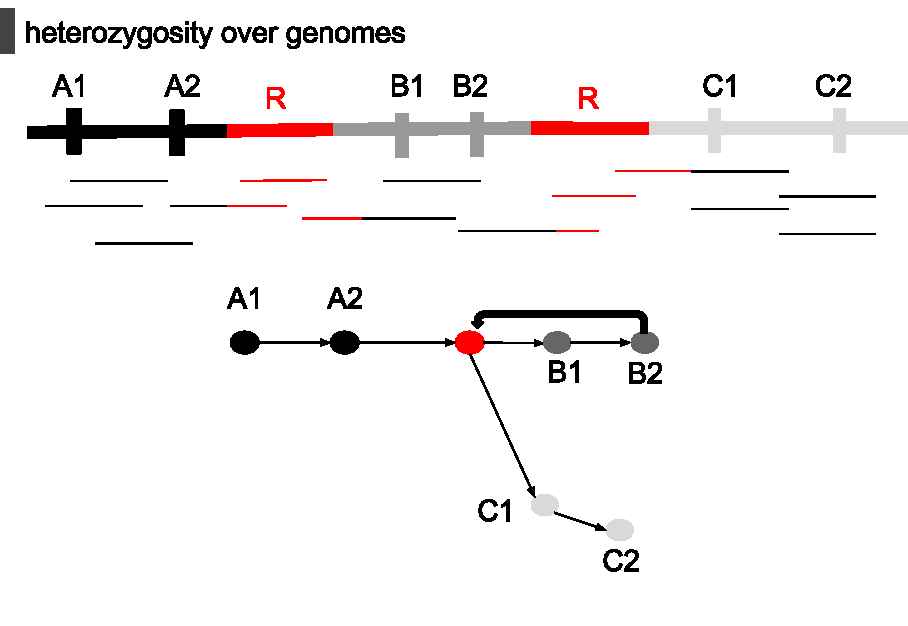
\includegraphics[width=\columnwidth]{repeats.pdf}
\caption{At the top, shown are the heterozygosity (in vertical bars) and repetitive regions (in red) over the genome. At the bottom, shown is the graph with nodes as heterozygous or repetitive region, and connections are based on the successive read overlap.
The graph has cycles because of repetitive region shown in R, and further also causes two branches.}
\label{fig:repeats}
\end{figure}

\textit{Repeats.} The repeats over the genomes causes branches or cycles in the assembly graphs and, therefore, makes graph more complex and break its linear chain properties.
This is illustrated in Figure~\ref{fig:repeats}. In this example, the repeat R causes cycle and branches in the graph.
The assemblers generally handle these repeats by making a guess as to which branch to follow.
Incorrect guesses create false joins (chimeric contigs) and erroneous copy numbers. 
If the assembler is more conservative, it will break the assembly at these branch points, leading to an accurate but fragmented assembly with fairly small contigs.
Furthermore, the maximal repeat resolution is decided based on the read-length. If there is a read that is long enough to span the repeat region, we say the repeat is resolvable.
Therefore, upcoming long-read sequencing technologies are a step forward to get better repeat resolved haplotypes.

\subsubsection{Haplotyping using assembly graph as reference}
In the most recent method for diploid genome assembly, Falcon Unzip method \citep{chin2016phased} uses the PacBio based assembly graph.
Falcon Unzip is a diploid-aware long-read assembler to assemble haplotype contigs or ``haplotigs'' that represent the diploid genome with correctly phased homologous chromosomes.
The pipeline is given in Figure~\ref{fig:falcon_unzip}. Falcon Unzip begins by using reads to construct a string graph that contains sets of ``haplotype-fused contigs'' as well as bubbles representing divergent regions between homologous sequences (Fig.~\ref{fig:falcon_unzip}a). 
Next, FALCON-Unzip identifies read haplotypes using phasing information from heterozygous positions that it identifies (Fig.~\ref{fig:falcon_unzip}b). 
Phased reads are then used to assemble haplotigs and primary contigs (backbone contigs for both haplotypes) (Fig.~\ref{fig:falcon_unzip}c) 
that form the final diploid assembly with phased single-nucleotide polymorphisms (SNPs) and structural variants (SVs).

\textit{Phasing using primary contigs.}
In Falcon Unzip, the reads are aligned to primary contigss and heterozygous SNPs (het-SNPs) are called by analyzing the base frequency of the detailed sequence alignments.
A simple phasing algorithm was developed to identify phased SNPs. 
Along each contig, the algorithm assigns phasing blocks where ``chained phased SNPs'' can be identified. 
Within each block, if a raw read contains a sufficient number of het-SNPs, it assigns a haplotype phase for the read unambiguously. 
Combined with the block and the haplotype phase information, it assigns a ``block-phase'' tag for each phased read in each phasing block.
Some reads might not have enough phasing information. For example, if there are not enough het-SNP sites covered by a read, it assigns a special 'un-phased tag' for each un-phased read.
The initial assembly graph is fused using phased reads and the haplotigs are generated in a greedy manner using local conservative approach.
% \todo{maybe add example how haplotigs from haplotype fused assembly graph works?}

\begin{figure}[t!]\centering
\includegraphics[width=\columnwidth]{{cropped_falcon-unzip}.pdf}
\caption{(a) An initial assembly is computed by FALCON, which error corrects the raw reads (not shown) and then assembles them using a string graph of the read overlaps. 
The assembled contigs are further refined by FALCON-Unzip into a final set of contigs and haplotigs. 
(b) Phase heterozygous SNPs and group reads by haplotype. (c) The phased reads are used to open up the haplotype-fused path and generate as output a set of primary contigs and associated haplotigs.}
\label{fig:falcon_unzip}
\end{figure}

To our knowledge, there is no work that phases directly from the assembly graph. 
\begin{gaps}
 Phasing bubbles directly from the assembly graph is an open problem. Additionally, the hybrid of multiple sequencing technologies such that using one technology that produces shorter, more accurate reads, and a second technology that delivers long reads, can lead to better quality haplotypes. 
\end{gaps}


Phasing using an assembly graph has several advantages over other approaches. For example, it is possible to phase larger blocks at once, because paths in an assembly graph can span multiple variants.
Moreover, it is easier to detect large structural variants, such as translocations and other rearrangements, in an assembly graph.
The graph-based approach provides a way to both accurately detect all types of structural variation and perform further downstream analyses.
\begin{example}
Figure~\ref{fig:ex_graph_approach} demonstrates the advantages of graph-based approach over contig-based Falcon Unzip method.
Consider four SNVs separated by two large SVs and there are four reads spanning these variants.
Falcon Unzip can not phase the reads $r_3$ and $r_4$ because they cover less than two SNVs, resulting in fragmented haplotigs.
In contrast, the graph-based approaches attempt to detect all types of SVs and can phase all the reads covering these SVs. In this example, reads $r_3$ and $r_4$ can also be phased because they cover SV1 and SV2, producing end-to-end haplotigs.
\end{example}
Therefore, the graph-based approaches are powerful to deliver more complete and contiguous haplotigs.

% \begin{figure}[t!]\centering
% 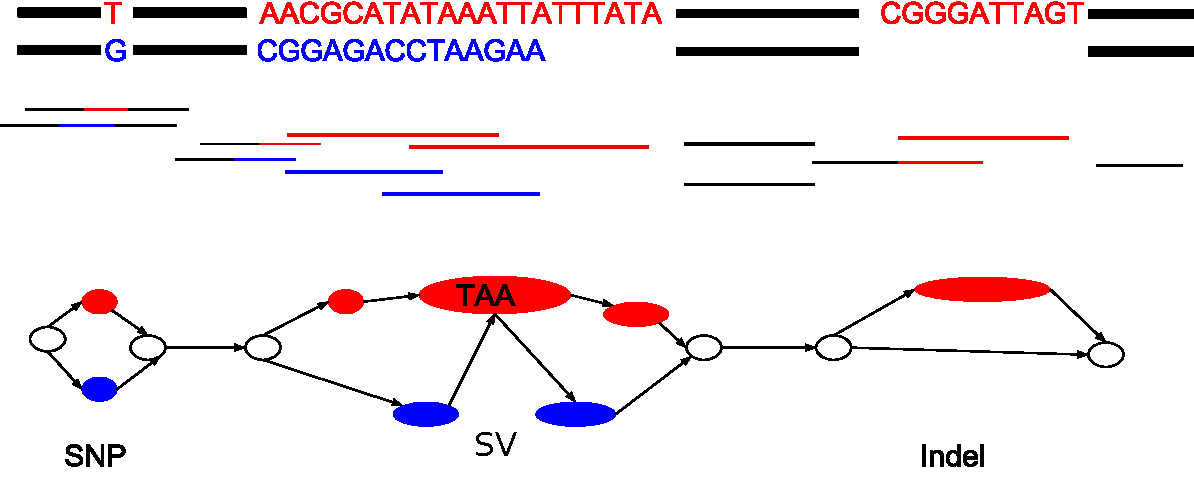
\includegraphics[width=\columnwidth]{ex_sv.pdf}
% \caption{Based on reads (middle) from the two sequences (top), the bubbles in the graph (bottom) show three different heterozygous structural variations; first is a SNV, second is a SV and third is an indel. }
% \label{fig:ex_sv}
% \end{figure}


\begin{figure}[t!]\centering
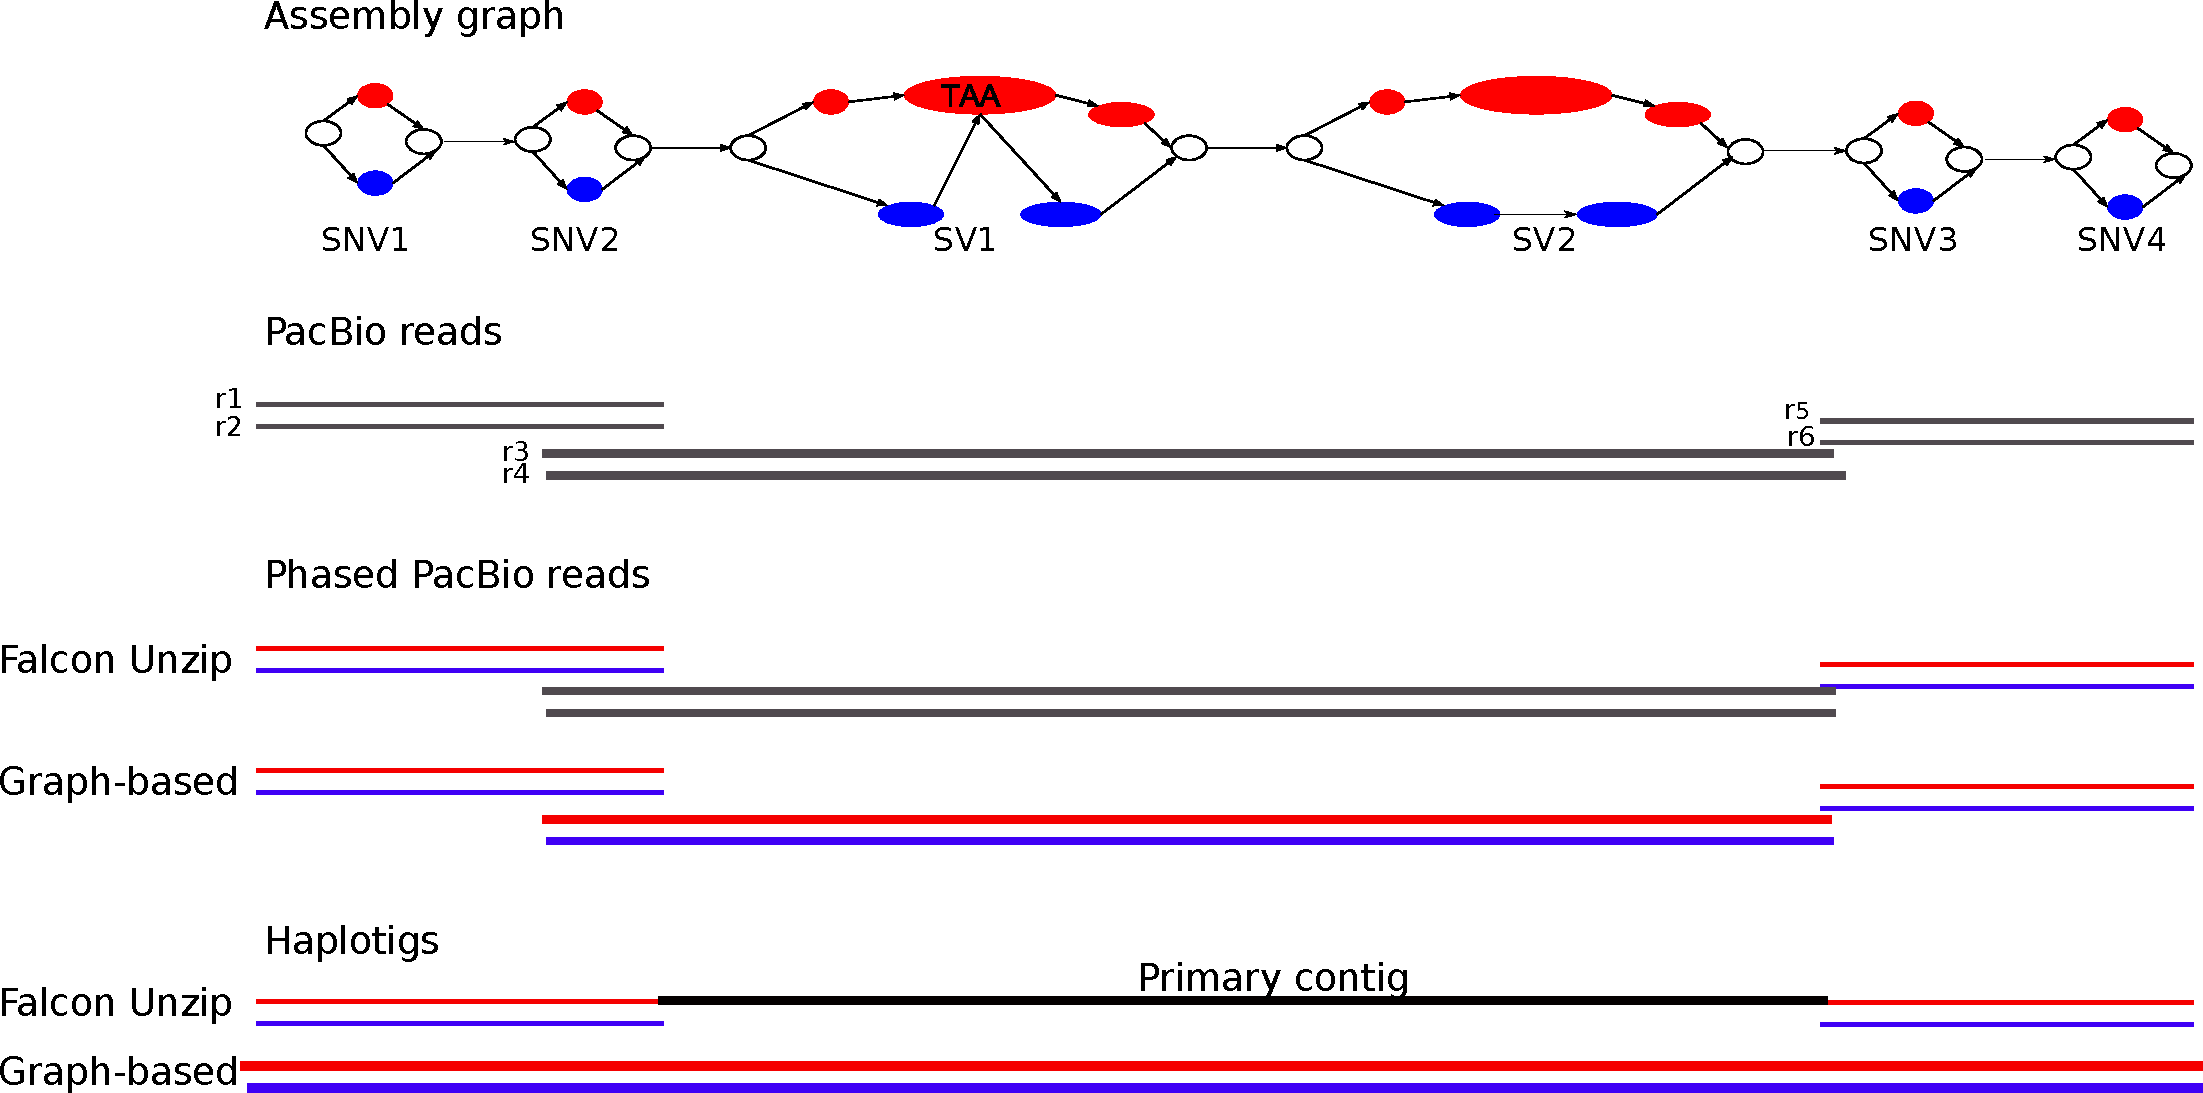
\includegraphics[width=\columnwidth]{ex_graph_approach.pdf}
\caption{Input: an assembly graph (top) (consisting of four SNVs and two SVs) and the PacBio reads $r_1, r_2, r_3, r_4, r_5, r_6$ (gray). Output: the phased reads (colored in blue and red) and haplotigs (bottom) using Falcon Unzip and our graph-based approach. Our graph-based phase all the reads, contrarily, Falcon Unzip don't phase the reads $r_3$ and $r_4$,  }
\label{fig:ex_graph_approach}
\end{figure}

\begin{figure}[t!]\centering
\includegraphics[width=\columnwidth]{{Marschall.152.fig.1}.pdf}
\caption{Seven SNP loci covered by reads (horizontal bars) in three individuals. Unphased genotypes are indicated by labels 0/0, 0/1 and 1/1. The alleles that a read supports are printed in white}
\label{fig:ex_pedigree}
\end{figure}


\subsection{Pedigree of genomes}
There is an another approach to haplotyping when we have sequencing datasets from the families of genomes.
In this, we can take advantage of two things: one is the sequencing data itself of each individual and the other is the principles of the Mendelian segregation of alleles in pedigrees. 
There are alleles that are specific to a single founding chromosome within a pedigree, which we refer to as lineage-specific alleles, are highly informative for identifying haplotypes that are identical-by-decent between individuals within a pedigree.
At the simplest level of a family trio (both parents and one child), very simple rules indicate which alleles in the child were inherited from each parent, thus largely separating the two haplotypes in the child.  
Nevertheless, genetic analysis cannot phase positions in which all family members are heterozygous. 
Furthermore, it is not always feasible to recruit the required participants for family-based studies. In the absence of a family context, molecular haplotyping is an excellent choice because it does not require DNA samples from other family members. 
The sequencing based haplotyping largely supplant the need for genetic analysis.
Haploscribe~\citep{roach2011chromosomal} is a suite of software scripts that phase whole-genome data across entire chromosomes by genetic analysis. Haploscribe implements a parsimony approach to generate
meiosis-indicator (inheritance state) vectors and uses a hidden Markov model (HMM) to deduce haplotypes spanning entire chromosomes.
To our knowledge, we are not aware of any method that uses both sequencing data and genetic inheritance principles in an integrative fashion to perform phasing.

\begin{gaps}
 Combining both principles of genetic inheritance and sequencing reads into one framework is not yet solved. Furthermore, the parameterized algorithm to solve this integrative framework is an important question.
\end{gaps}

\begin{example}
 To illustrate the motivation to combine genetic and read-based haplotyping, the corresponding \MEC instance for a single genome is shown in Figure~\ref{fig:ex_pedigree}. 
There are seven SNP positions covered by reads in three related individuals. 
It illustrates how the ideas of genetic and read-based haplotyping complement each other. 
All genotypes at SNP 3 are heterozygous. 
Thus, its phasing cannot be inferred by genetic phasing, that is, using only the given genotypes and not the reads. SNP 4, 
in contrast, is not covered by any read in the child. When only using reads in the child (corresponding to single-individual read-based phasing), 
no inference can be made about the phase of SNP 4 and neither about the phase between SNP 3 and SNP 5. 
By observing that all seven child genotypes are compatible with the combination of brown and green haplotypes from the parents, 
however, these phases can be easily inferred. This example demonstrates that jointly using pedigree information, genotypes and sequencing reads is very powerful for establishing phase information.
\end{example}

\section{Outline of our contributions}
In the above section, we highlighted four ``open problems'' in the diploid genome assembly of NGS data:
\subsection{Open Problems}
\begin{enumerate}
 \item Approximation status of \GMEC.
 \item Integrative framework for haplotyping using different types of datasets.
 \item Denovo diploid genome assembly.
 \item Phasing pedigree of genomes.
\end{enumerate}

\subsection{Issues we address}
To address those problems, we will present new algorithmic approaches. 
\begin{enumerate}
 \item In the first chapter, we present dynamic programming based algorithm to prove the near-polynomial approximation status of \GMEC.
 \item In the second chapter, we present a parameterized algorithm to solve \MEC instances integatively from different datasets.
 \item In the third chapter, we introduce new way to represent the assembly graph and futher, finding long read paths in the graph based on different types of datasets, helps in better phasing. 
 \item In the forth chapter, we present a integrative framework to solve sequencing-based and genetic haplotyping, helps to generate complete and accurate haplotypes.
\end{enumerate}


% 
% 
%  
% 
% \todo{cover these issues in approaches}
% \subsection{Diploid genome assembly hardness}
% \begin{itemize}
% \item Theoretical approximation gurantee on gapless-MEC. It is important because even for high coverages, we can solve it in polynomial time approximately.
%  \item integrating datasets to produce more accurarte and complete
%  \item non-reference denovo based, can not detect large SVs, directly from graph, hybrid
%  \item pedigree of genomes
% \end{itemize}
% 
% \subsection{Goals and achievements}
% \begin{enumerate}
%  \item DNA genomes ranging from small yeast like genome to larger ones like human.
%  \item end-to-end full genome sequences
%  \item efficient algorithms to generate optimal or near-optimal solution.
% \end{enumerate}
% 
% 
% 
% 
% \subsection{Outline of our contributions}
% \begin{enumerate}
%  \item Chpater 1 consists of ...
%   \item Chpater 2 consists of ...
%    \item Chpater 3 consists of ...
% \end{enumerate}






